\chapter{Implementation} \label{Impl}
The implementation of the system is oriented at following the V-Modell. In section \ref{Require}, the requirements of the designed system are defined. This section is followed by a description of the system architecture of the vessels \ac{GNC} system and peripherals in \ref{Archi}. The part of the architecture that is further detailed in the implementation is described hereafter. The system specification in section \ref{Spec} discusses the possible hardware, the simulation environment and the software framework used to realize the defined architecture. The software modules and its interdependencies both for the simulation and the software framework are defined in section \ref{ModuleDes} and are followed by a more detailed description and the implementation in section \ref{ModuleImp}. 

\section{Requirements}\label{Require}
 This section describes the requirements that derive from the use case of the system. The requirements are separated in the three main categories safety considerations in subsection \ref{Regulations} and hardware and software requirements in subsection \ref{ReqHardSoft}.
 \subsection{Regulations and safety}\label{Regulations}
 \begin{figure}[h]
 	\centering
 	\begin{tikzpicture}
 	[node distance = 1cm, auto,font=\footnotesize,
 	% STYLES
 	every node/.style={node distance=3cm},
 	% The comment style is used to describe the characteristics of each force
 	comment/.style={rectangle, inner sep= 5pt, text width=4cm, node distance=0.25cm},
 	% The force style is used to draw the forces' name
 	force/.style={rectangle, draw, fill=black!10, inner sep=5pt, text width=2.5cm, minimum height=1.1cm,  text badly centered}]
 	
 	% V model box centre
 	\node [force,] (Code) {Code\\implementation};
 	%left
 	\node [force, above left = 0.5cm of Code] (Modul) {Modul\\Design};
 	\node [force, above = 0.5cm of Modul] (System) {Software\\System};
 	\node [force, above = 0.5cm of System] (Archi) {Software\\Architecture};
 	\node [force, above = 0.5cm of Archi] (Spezi) {Spezification\\Software Safety};
 	%right
 	\node [force, above right = 0.5cm of Code] (Modultest) {Test\\Modules};
 	\node [force, above = 0.5cm of Modultest] (Integration) {Integrationtest\\Modules};
 	\node [force, above = 0.5cm of Integration] (Integrationparts) {Integrationtest\\Parts};
 	\node [force, above = 0.5cm of Integrationparts] (Validation) {Validation\\Software};
 	%left of v modell
 	\node [force, left = 0.5cm of Spezi] (Req) {Electric/Software\\Safety};
 	\node [force, left = 0.5cm of Archi] (ArchiEl) {Electric/Software\\System Design};
 	% Draw the links between sensor forces, HMI and Actuators
 	\path[<->,thick]
 	% Vmodell and one addition at end
 	(Code) edge (Modul)
 	(Modul) edge (System)
 	(System) edge (Archi)
 	(Archi) edge (Spezi)
 	(Code) edge (Modultest)
 	(Modultest) edge (Integration)
 	(Integration) edge (Integrationparts)
 	(Integrationparts) edge (Validation)
 	(ArchiEl) edge (Archi);
 	%dotted lines of Vmodell
 	\path[<->,thick, dashed]
 	(Modul) edge (Modultest)
 	(System) edge (Integration)
 	(Archi) edge (Integrationparts)
 	(Spezi) edge (Validation);
 	% Draw lines right and left 
 	\path[->,thick]
 	(Req) edge (Spezi)
 	(Req) edge (ArchiEl);
 	
 	\end{tikzpicture} 
 	\caption{Systematic development of safety related software with the V-Model after \cite{DIN_1}.}
 	\label{fig_VModel}
 \end{figure}
 The design of a technical system has to be conducted by taking into account technical regulations. Both the EU and \ac{IMO} developed regulations for the requirements of testing \ac{MASS}. Among the regulations in the interim guidelines of the \ac{IMO} is the demand for an adequate human-system interface and a human centred design of a \ac{MASS}. Furthermore, information that is related to the vessels internal state and the data upon which the automated system judges the scene should be made available to any personnel involved in the \ac{MASS} trial \cite{IMO_MASS}. The regulation published by the EU takes into consideration the aforementioned regulation of the \ac{IMO} and highlights the  ability of the applicant of the \ac{MASS} trial to maintain a meaningful human control at any time during the test or trial with the ability to abort the trial \cite{EU_MASS}.\\
 
 Regarding the detailed design process, there are many organizations that develop standards for safety related software with the \ac{IEEE} and the \ac{IEC} considered as the most important organizations \cite{OverviewReg}. For more detailed specifications of the software requirements in programmable electronic safety related systems in Germany, the \ac{VDE} 0803-3 \cite{DIN_3} can be acquired which is related to \ac{IEC} 61508. Section 7.1 to 7.9 describe the requirements of a software safety life cycle. General information are given (7.1) and safety requirements specified (7.2). The validation of software is described (7.3) and the software development process related to safety aspects explained (7.4). The document continuous with the integration of software and electronic parts (7.5), modification processes (7.6), the software validation (7.7) and software modification (7.8) and verification (7.9). It is stated, that every model of a software safety life cycle that full fills the requirements of the document is allowed to be used with an example given by the V-Model as depicted in figure \ref{fig_VModel}. The figure describes from the upper left to the upper right the states of a development process related to the safety of software and it becomes clear, that embedding this model in a traditional V-model development process is possible. First, the electrical and software safety requirements are determined to design the electrical and software system upon which the software architecture relies. Also, the specification of the software safety can be derived from this requirements. During these steps, the software is validated and integrations tests of the software architecture are defined. The software system and module design takes place hereafter with the integration test and module test specified and applied simultaneously. The most detailed level of the design is the code implementation. The model as proposed in \ac{VDE} 0803-3 is intended to be applied on large projects, therefore steps can be merged for the application in small projects.\\
 
 Of special interests is section 7.4 in this document as it details the software design and development process with subsection 7.4.3 specifying the requirements for the design of a software architecture. The design of the system should be without faults in the concept, easily comprehensible and display a deterministic behaviour. The implementation of the design is required to be testable and has to be fault tolerant even in the case of external events. The responsibility for the software as well as the architecture of the design and modifications shall be documented (7.4.3.1-3). The document is continued by subsection 7.4.5 comprising the requirements for a detailed software system design. The responsibility for the software as well as the intended design of the system with related electrical parts and a plan for the safety validation of the system has to be documented (7.4.5.1-2). The software shall be programmed in such a way, that a modular, testable and changeable code is obtained and every system is divided into several more detailed submodules (7.4.5.3-4). Tests for the integration shall be specified in order to full fill the required safety integrity level. Every software code that is implemented shall be tested as specified in section 7.4.6.\\
  
 It is noted, that an according regulation for the development and use of programmable electronic systems in marine applications \cite{ISO} by the \ac{ISO} exists but is not used in favour for the more specific \ac{IEC} 61508 , which is referred to in the \ac{ISO} document for detailed information regarding the design process \cite{LearningAuto}.
 
 \subsection{Hardware and software} \label{ReqHardSoft}
 To enable a \ac{USV} to percept its environment, suitable sensors have to be found and ideally fused into a fault resistant representation of a present scene by the navigation subsystem.  The navigation subsystem that integrates this sensors is required to be modular to allow the system to be updated independently from other subsystems and thus provide situational awareness in changing scenes. The exchange of information with other subsystems should be ensured and a focus has to be laid on the user of the system \cite{ReqNav}. The resulting data of the navigation subsystem can be utilized in a subsequent step to control the \ac{USV} actuators in a way that serves the objectives of the planned mission. Different sensors are proposed to be utilized in a \ac{GNC} system \cite{Liu2016}. The navigation subsystem is supposed to detect obstacles and determines its position both globally and in relation to the \ac{USV}. Therefore, for long range obstacle detection, \ac{RADAR} is most suitable whereas for short distances and a higher distance resolution and accuracy \ac{LIDAR} serves the purpose. To classify objects, cameras can be used. At very close range, ultrasonic sensors are an affordable solution for obstacle detection. The global position of a \ac{USV} can be determined by \ac{GNSS} \cite{EnvPerc}. To synchronize the mission goals with the control centre a connection to the guidance subsystem is required. Furthermore, to archive given control objectives, the influences of environmental disturbances have to be measured by a wind gauge which provides both wind direction and velocity. A water speed sensor and a three dimensional \ac{IMU} serves as a feedback for the control subsystem. Ideally, the sensors can be connected to a system which allows data to be manipulated, broadcasted and send to a control station on request.\\
 
 \section{System Architecture}\label{Archi}
 
 Figure \ref{fig_systemGNC} incorporates a comprehensive system diagram of a vessels \ac{GNC} system with a software framework functioning as the middleware on a processor unit. The peripheral sensors are connected to the interface of the processor unit. The sensors data can be filtered and processed to such an extent that they suffice the data rate to the control centre and can be send to it via a connection of choice. A \ac{HMI} connected to the control centre provides the possibility to send instructions to the operating system of the vessel and thus allow the full control over the system. Consequently, a connection to the actuator control enables the applicant to access relevant functions. The actuators sensors provide the control subsystem and the control centre with data of its operational status. The system architecture as depicted allows for the selection of either real sensors or virtual sensors in conjunction with a simulation environment. The simulation can be run on a different processing unit than the software framework. However, given sufficient processing power, calculations for both systems can be conducted on one system as well.
  
 \begin{figure}[h]
 	\centering
 	\begin{tikzpicture}
 	[node distance = 1cm, auto,font=\footnotesize,
 	% STYLES
 	every node/.style={node distance=3cm},
 	% The comment style is used to describe the characteristics of each force
 	comment/.style={rectangle, inner sep= 5pt, text width=4cm, node distance=0.25cm},
 	% The force style is used to draw the forces' name
 	force/.style={rectangle, draw, fill=black!10, inner sep=5pt, text width=2cm, text badly centered}]
 	
 	% Linux box with comment
 	\node [rectangle, draw, fill=black!5, minimum height=2cm, minimum width=4cm, dashed ] (Linux){Linux};
 	\node [comment, below=-0.5 of Linux, text centered] (comment-Linux) {Processing Unit A};
 
 	
 	% ROS box
 	\node [force,minimum height=1.2cm] (ROS) {Software\\Framework};
 	
 	% Sensor boxes
 	\node [force, left= 0.5 of Linux] (RealSensors) {Real Sensors};
 	
 	% Control centre box
 	\node [force,minimum height=1.2cm, above= 1cm of ROS] (Control) {Control Centre};
 	\draw [<->,thick](Control) -- (Linux) node [] {};
 	
 	% HMI
 	\node [force, right=1cm of Control](Human) {\ac{HMI}};
 	\draw [<->,thick](Control) -- (Human) node [] {};
 	
 	% Acutators
 	\node [force, right=1cm of Linux](Actuators) {Actuators};
 	 	
 	% Actuators sensor
 	\node [force, right=1cm of Linux, below= 0.25cm of Actuators](Propulsion) {Sensorsystem \newline Propulsion};
 	\draw [->,thick](Propulsion) -- (Linux) node [] {};
 	\draw [<-,thick](Propulsion) -- (Actuators) node [] {};
 	
 	% ComputerB
 	\node [rectangle, draw, fill=black!5, minimum height=2cm, minimum width=5cm, dashed, below =0.5cm of Linux ] (ComputerBl){};
 	\node [comment, below=-0.5 of ComputerBl, text centered] (comment-ComputerBl) {Processing Unit B};
 	\draw [<->, thick] (ComputerBl) -- (Linux) node []{};
 	
 	% Unity, Sensor box
 	\node [force,left= -2.45cm of ComputerBl] (Unity) {Simulation Environment};
 	\node [force,right=-2.45cm of ComputerBl] (Sensor) {Virtual Sensors};
 	
 	% Draw the links between sensor forces, HMI and Actuators
 	\path[->,thick]
 	(RealSensors) edge (Linux)
 	(Linux) edge (Actuators);

 	\end{tikzpicture} 
 	\caption{System diagram of the \ac{GNC} system}
 	\label{fig_systemGNC}
  \end{figure}

\section{System Specification} \label{Spec}
Referring to the designed system architecture in section \ref{Archi}, in this section the described systems of the architecture are specified. A focus is on the peripheral devices and the processing unit, that are outlined in subsection \ref{PeriDev}, followed by the selection of a central software framework in subsection \ref{Softframe}. Finally, the virtual environment is specified in subsection \ref{virtuenv}.

\subsection{Peripheral Devices and Central Processing Unit} \label{PeriDev}
The sensors described in the following are not implemented and used in an experimental verification but its defined characteristics are important for the subsequent design and implementation of the virtual sensors. They were however chosen with respect to the appliance at hand and an implementation in a real environment is encouraged. The choice of sensors is considerably reduced by the exclusion of proprietary interfaces as these can not be connected to a third party or open source solution and thus allow only very restricted access to the sensors data. An example is given by \ac{RADAR} solutions which almost always relay on the manufacturers choice of displays and therefore do not allow the data to be filtered, clustered or otherwise manipulated. Additionally a \ac{SDK} can be bought only on request, with not further specified predefined functions and executable only on the manufacturers choice of operating system. Due to this restrictions and the recent progress in solid state \ac{RADAR} solutions in the automotive field \cite{ResRADAR}, it has to be taken into consideration to use such a sensor in addition to a \ac{LIDAR} system.\\

The Aptive ESR 2.5 \cite{AptivESR} is such a automotive \ac{RADAR} sensor. It applies a millimetre wave radiation, this having a wavelength of around 80Ghz, to the environment and thereby senses up to 64 targets within a distance of 174m in long range mode. In addition to the long range mode with a \ac{FOV} of $\pm10^{\circ}$, a mid range mode with a range of 60m and a \ac{FOV} of $\pm45^{\circ}$ provides a higher degree of spatial width. The Aptive ESR 2.5 can be integrated into \ac{ROS} with an \ac{API} for \ac{CAN} provided by the company AutonomousStuff. Additionally to the \ac{CAN} interface which only provides data about extracted obstacles, an Ethernet interface gives access to the raw data of the \ac{RADAR}. To ensure the detection of obstacles further away, the Garmin GMR Fantom 54 \ac{RADAR} is used. It radiates with a power of 50W and has a range from 6m to 72 nautical miles. For closer distances of up to 100m , the Velodyne Puck \cite{VelodynePuck} provides a 3D point cloud of environmental objects with 300000 points per second and for ranges of up to 7.5m, the SEN0313 Ultrasonic sensor \cite{UltrasonicA01} gives access to analogue distance measurements. The BFS-U3-13Y3C-C 1.3MP Blackfly camera from the manufacturer Flirr \cite{Blackfly} allows for the classification of detected objects. The MTi-680G by XSens \cite{XSens}, an integrated \ac{IMU} and \ac{GNSS} unit, allows vessel localization and movement detection. Wind speed and direction can be measured with the WS200-UMB ultrasonic anemometer by Lufft \cite{Lufft}. The advantage of an ultrasonic wind gauge solution can be found in the absence of moving parts and thus an extended lifecycle. A wireless transmission to additional devices in the network is realized by the FL WLAN 1101 by Phoenix Contact \cite{Phoenix_WLAN}. An overview of suitable sensors is given in table \ref{tab_sensor}. In the table, the sensor type is horizontally followed by the product name of the chosen sensor and an estimated price as well as the interface the sensor uses to transmit data.\\

To integrate the sensors and connect its data, a central hardware solution has to be found. The Jetson AGX Xavier hardware specifications qualify it as the central data processing unit. The Xavier Development Kit provides a development platform with many standard hardware interfaces that results in a highly flexible and extensible platform for rapid prototyping. It uses a maximum power of 30W for its own supply and can supply external peripheral devices with an overall power of 35W. The Xavier Development Kit can be interfaced via USB, UART, I2C, CSI-2, Ethernet and a variety of other ports. It is run by a derivative of the operating system Linux Ubuntu. As the hardware platform hosts a powerful \ac{GPU} with according libraries such as OpenCV and TensorRT and a Multimedia \ac{API}, it is a suitable solution for sensor integration and data processing \cite{Xavier}.

\begin{table}[H]
	 \centering	
		\caption{Sensors for environment detection}
		\begin{tabular}{l l l } 
			\toprule
			Type  & Name  & Interface \\[0.25ex]
			\midrule
			RADAR&Aptive ESR 2.5 & CAN/Ethernet\\	
			RADAR & GMR Fantom 54 & Ethernet \\	
			LIDAR & Velodyne Puck & Ethernet \\	
			IMU &\multirow{3}{*}{MTi-680G}& \\  
			GNSS & &CAN\\
			Velocity&& \\
			Windspeed&WS200-UMB &  RS485\\ 
			Camera &Blackfly 1.3 MP& USB 3.1\\
			Processor & Jetson AGX Xavier  & various\\	
			Ultrasonic  & SEN0313  &  digital\\	
			WLAN & FL WLAN 1101& Ethernet \\
			\bottomrule
		\end{tabular}
	\label{tab_sensor}
\end{table}

\subsection{Software Framework} \label{Softframe}

To integrate the sensor and provide a middleware to execute the \ac{GNC} system, the frameworks \ac{ROS}, \ac{CARACAS} and \ac{MOOS-IvP} are taken into consideration. These system platforms facilitates the effort to program the required functions with predefined libraries and communication structures. 
\begin{itemize}
	\item The \ac{CARACAS} architecture is available on request for research projects and is potentially applicable on diverse robotic systems. The system is divided into three agents that interact with each other and a data storage that hosts a world model. The objective of the agents is to provide the robotic system with the capabilities of both deterministic reactions to unanticipated occurrences and re-planning in the event of changes in goals and resources. The focus therefore is on the guidance subsystem of the \ac{GNC} system \cite{CARACAS}.
	\item \ac{MOOS-IvP} is an open source project and specifically intended for the application in unmanned marine vehicles. An autonomy system, which can be referred to as the guidance subsystem, runs the autonomous decision making helmet \ac{MOOS-IvP} which is connected with an input to the data of a navigation subsystem and with an output of data of the control system (figure \ref{fig_MOOS}). Therefore, it is decoupled from the platforms hardware and does not require any specification of how the navigation and control subsystem is implemented \cite{MOOS}.
	\item  \ac{ROS} is an open source software which is developed with the objectives of modularity, usage of a peer to peer structure and being based on tools. A low level device control provides drivers for peripheral devices and a hardware independent architecture allows \ac{ROS} to be run on a wide variety of devices. Community based libraries provide methods for sensor data processing and visualization, obstacle detection, mapping and path finding \cite{ROS}. As the sensor integration into the \ac{GNC} system is vital in the design of a new robotic platform, \ac{ROS} can be evaluated as a middleware software.
\end{itemize}	

\begin{figure}
	\begin{centering}
		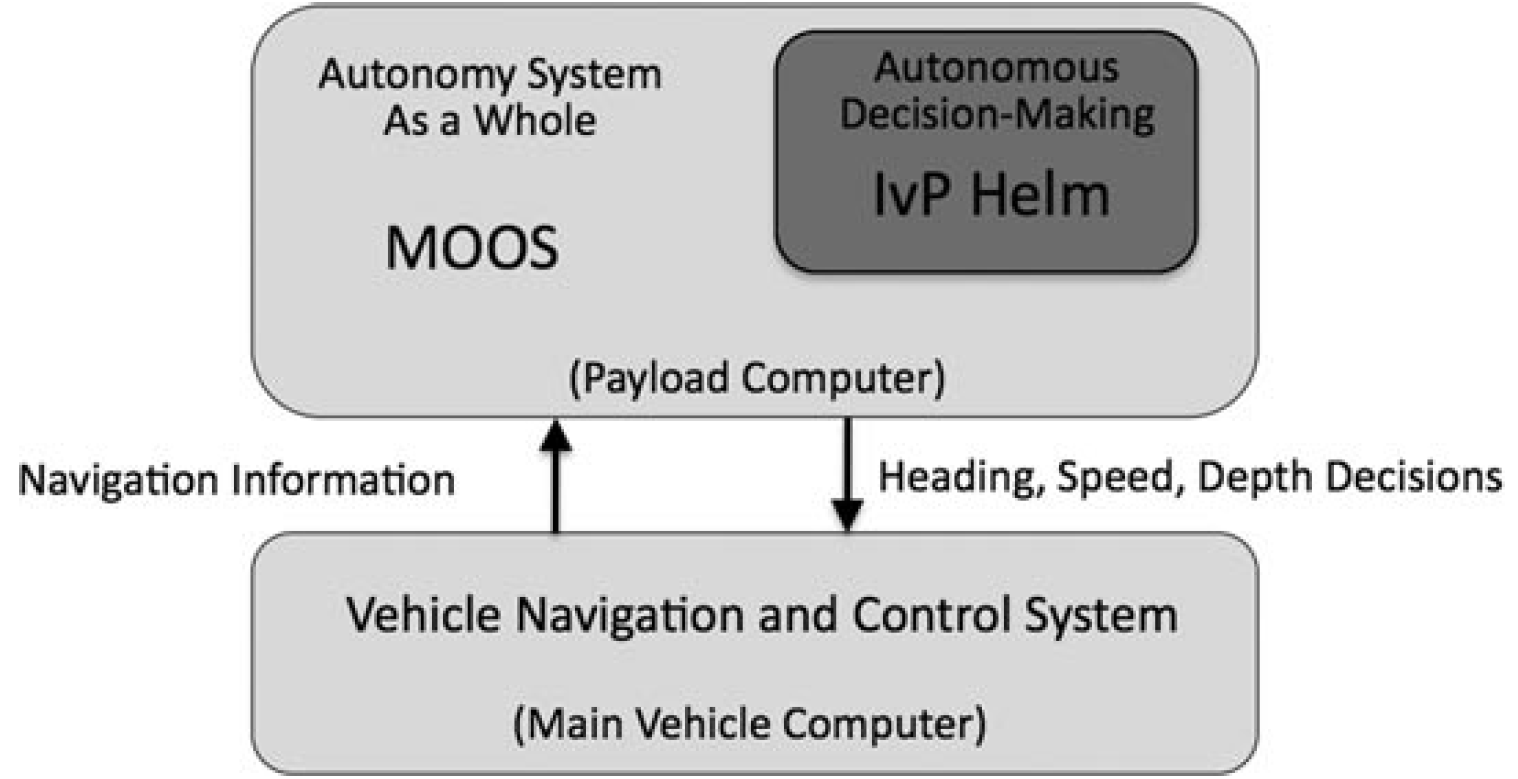
\includegraphics[width=10cm,keepaspectratio]{Bilder/MOOS.PNG}
		\caption{System diagram of the \ac{MOOS-IvP} architecture after \cite{MOOS}. The navigation and control system is physically decoupled from the autonomy system and is not further specified.}
		\label{fig_MOOS}%Label für das Referenzieren 
	\end{centering}
\end{figure}

With two different implementations of  \ac{ROS}, namely ROS1 and ROS2, the choice has to be made which of them is best suited to the application at hand. Developed since 2007, ROS1 provides a comprehensive set of packages \cite{ROSExample} and is supported until 2025. Therefore, four more years of active development is ahead of the current long term supported derivation, which is \textit{Noetic Ninjemys}. With the four years ending, adding new hardware can proof difficult because of the lack of drivers, however the system as developed before would continue to be functional. ROS1 is not build with native real time support \cite{ROSPerform}. Released with an first beta version in 2016, ROS2 still needs resources to implement interface functions and migrate packages from ROS1. For example Unity features are not supported at all and Gazebo is supported only partially in ROS2. However, ROS2 provides real time characteristics (note that real time capability depends on the underlying operating system as well as on the device driver \cite{ROSRealtime}), is suitable for small embedded platforms and can be run not only on Linux. It implements a \ac{DDS} in exchange for the ROS1 message transport system. \ac{DDS} follows an industry standard and provides real time communication by various configurations such as deadline, reliability and durability specifications \cite{ROSDDS}.\\

To further verify \ac{ROS} as a middleware for interfacing sensors and process its data, the performance of the software in situations with a high amount of data traffic has to be evaluated. In figure \ref{fig_ROSPerform}, the data latency [$ms$] with respect to the data size [$byte$] is plotted. Two machines with an Intel Core i5 are used for remote and local transmission of a string typed message in a 10Hz interval. The latency difference for data of 4Mb in figure \ref{fig_ROS1vsROS2} for ROS1 Indigo and ROS2 Cement can be neglected in comparison to the difference of remote and local data transmission with a latency of about 80ms and 5ms respectively. Thus, when dealing with large datasets as resulting from for example \ac{LIDAR} point clouds, processing data locally is to be preferred over the transmission of data to another data processing device. The performance of local data transmission in \ac{ROS} is detailed in figure \ref{fig_ROS1vsROS2Intra}. Performance of data transmission by a pointer (referred to as nodelet in ROS1 and intra in ROS2), by a node via \ac{TCP} (referred to as local), by the OpenSplice implementation of \ac{DDS} set to reliable and in between ROS1 and ROS2 are compared. The performance of a nodelet in ROS1 exceeds the other transmission modes with a latency of less then 2ms at a data size of 4Mb.  It is followed by a ROS1 node with less than 4ms. The performance of the communication between ROS1 and ROS2 with 5ms latency at only 1Mb of data size is the least performing transmission method \cite{ROSDDS}. As for a real time system, not only the transmission time, but the compliance with predefined timing deadlines is important, in figure \ref{fig_ROS2RT} and \ref{fig_ROS2RTOver} the number of messages that missed its deadlines are displayed. The tests are conducted with two different machines that run Linux with a PREEMPT-RT patched kernel, which is a real time kernel implementation for Linux. The \ac{RTT} from one machine to the other are measured with the ROS2 profile "best-effort reliability" and three different \ac{DDS} implementation in each test. In figure \ref{fig_ROS2RT} the message latency is plotted against the number of samples with that latency. Even with a system traffic of 40Mbps and the processor under load, three, zero and five samples in accordance with the \ac{DDS} preferences missed the preset deadlines over a test time of 12h and of a total of 4320000 samples. In figure \ref{fig_ROS2RTOver} the same test was conducted but only over a time period of 10 min and with an increased traffic of 80 Mbps. This results in missed deadlines of 1470, 1799 and 570 missed deadlines dependent on the \ac{DDS} settings with a total of below 60000 send samples. This can be considered as not sufficient for real time appliances \cite{ROSRealtime}.\\

It can be concluded, that in having a supported deterministic behaviour and a long support window, the advantage of ROS2 outweighs the disadvantage of lacking development resources in the appliance to the middleware of the \ac{GNC} system. In addition the interface to the game engine Unity3d is proven to work for ROS2 as well as ROS1 with only small changes in the workflow. The drawback of a less extended development community is presently becoming smaller as the industry more and more supplies software and support for ROS2. This is a trend that can be expected to grow in the future. Therefore, ROS2 is chosen as the middleware for the implementation of the \ac{GNC} system.


%The test conducted in \ref{fig_ROS1Perform} and \ref{fig_DDSPerform} are performed on the \ac{ROS} distribution Kinetic Kame and the eProsima Fast RTPS \ac{DDS} implementation respectively. To measure the response time, the \ac{RTT} is measured by an echo reply of the initial message. The \ac{RTT} is measured while the system is in idle mode, during an artificial generated \ac{CPU} load and traffic in the network. With focus on the messages of about 32 kByte, message transmission with \ac{DDS} results in less response time than using \ac{ROS}. However it has to be stated, that in \ac{ROS}, 75$\%$ of messages have response times below 2$ms$ and the average difference between the response time with a high network load compared to \ac{DDS} is below 100 $\mu s$. With the system in idle and CPU load mode, this value rises to 400$\mu s$ and 700$\mu s$. Even with 32kbyte of data, that can be considered to be small compared to the data generated by 3D sensors, the response time varies widely with differences of up to 1.5$ms$.\\

\begin{figure}
	\centering
\begin{subfigure}[b]{0.49\textwidth}
	\centering
	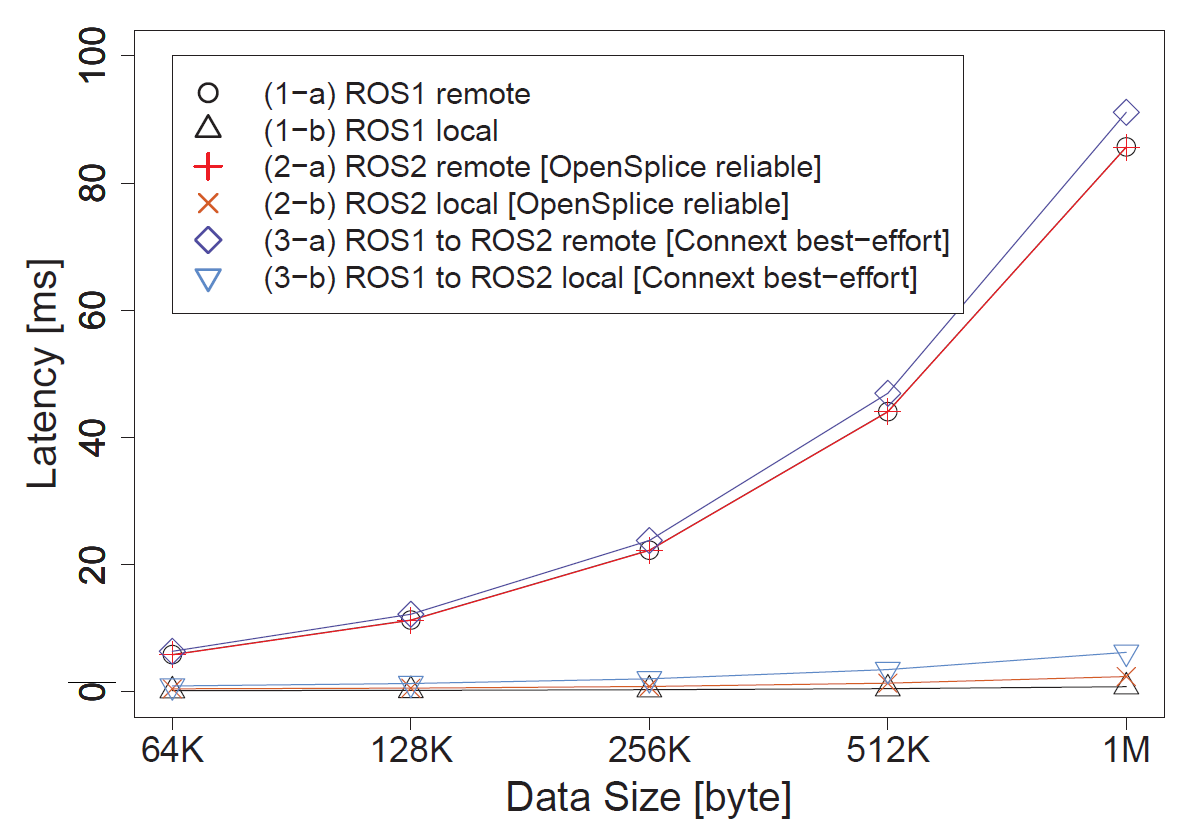
\includegraphics[width=\textwidth]{Bilder/PerformEndtoEnd.PNG}
	\caption{Latency in ROS1 and ROS2 in $[ms]$ for remote/local data transmission of 64 Kbyte to 1 Mbyte by \cite{ROSDDS}.}
	\label{fig_ROS1vsROS2}
\end{subfigure}
\hfill
\begin{subfigure}[b]{0.49\textwidth}
	\centering
	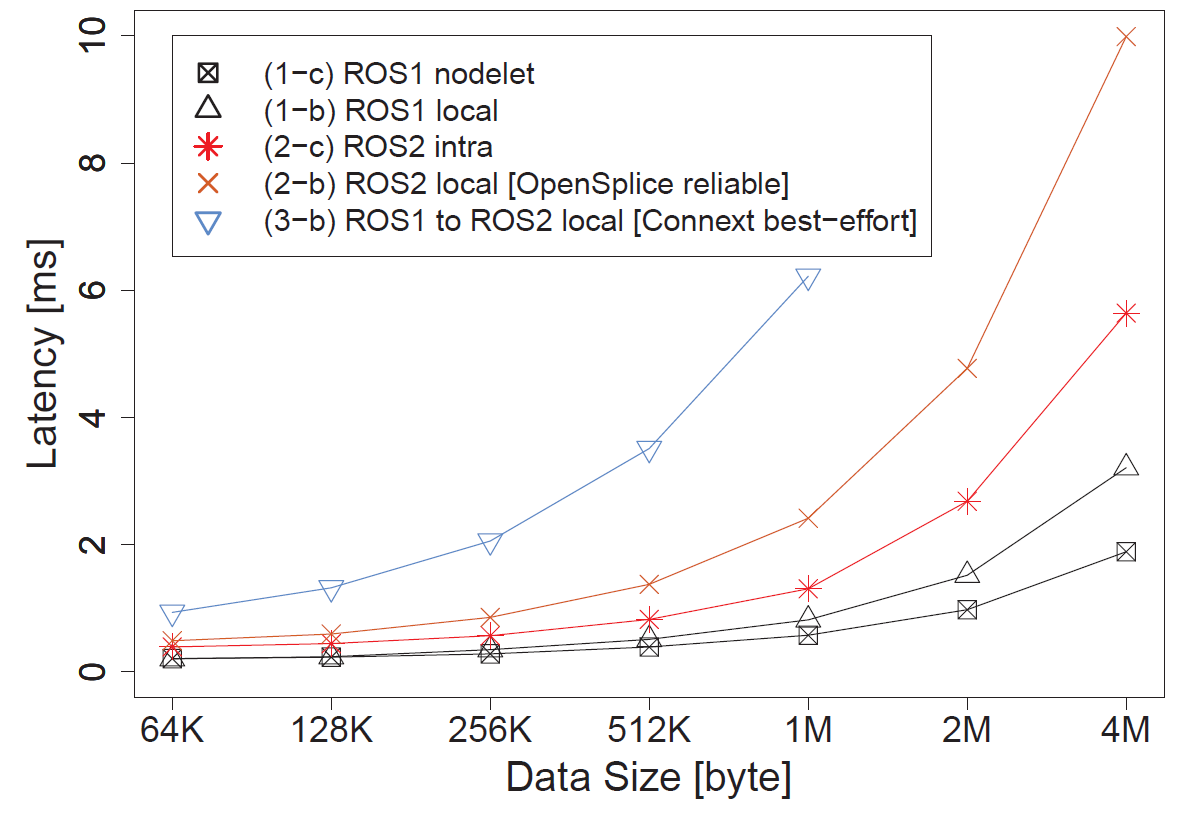
\includegraphics[width=\textwidth]{Bilder/PerformIntra.PNG}
	\caption{Latency in ROS1 and ROS2 in $[ms]$ for local data transmission of 64 Kbyte to 4 Mbyte by \cite{ROSDDS}.}
	\label{fig_ROS1vsROS2Intra}
\end{subfigure}
	\begin{subfigure}[b]{0.49\textwidth}
		\centering
		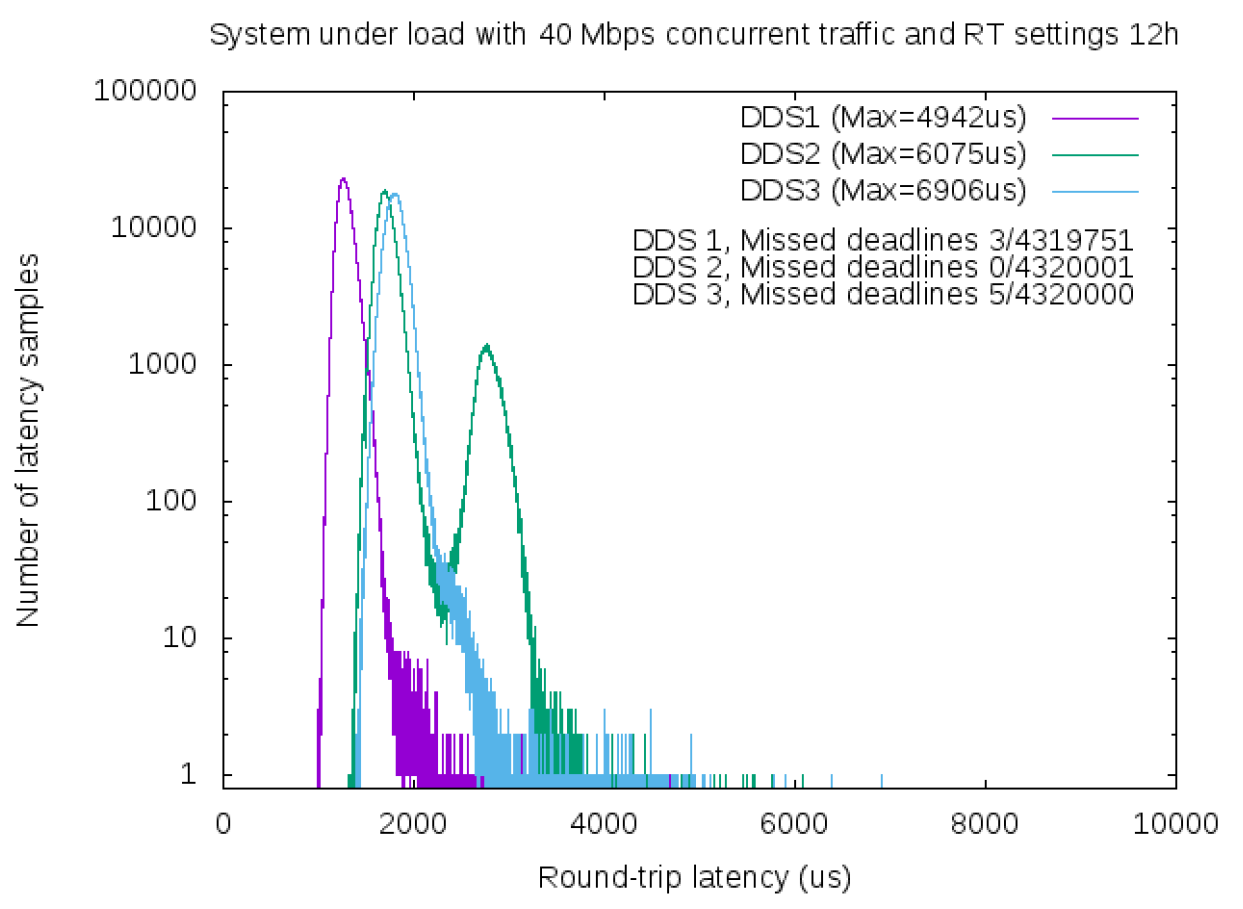
\includegraphics[width=\textwidth]{Bilder/ROS2Realtime.PNG}
		\caption{ROS2 round-trip latency in $[\mu s]$ for three different timing deadlines for 40Mbps in 12h under \ac{CPU} load by \cite{ROSRealtime}.}
		\label{fig_ROS2RT}
	\end{subfigure}
	\hfill
	\begin{subfigure}[b]{0.49\textwidth}
		\centering
		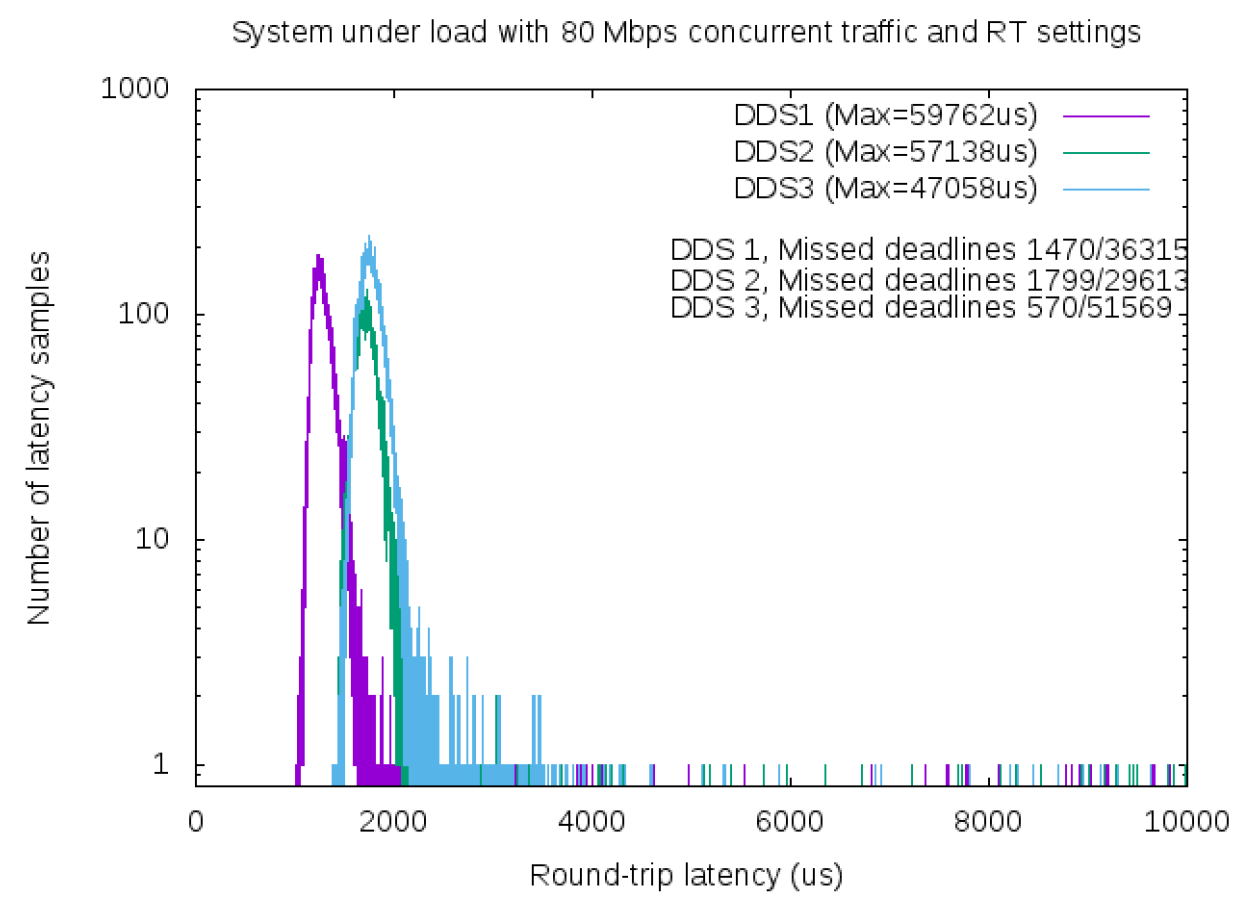
\includegraphics[width=\textwidth]{Bilder/ROS2RealtimeOver.PNG}
		\caption{ROS2 round-trip latency in $[\mu s]$ for three different timing deadlines for 80Mbps in 10min under \ac{CPU} load by \cite{ROSRealtime}.}
		\label{fig_ROS2RTOver}
	\end{subfigure}	
%	\begin{subfigure}[b]{0.49\textwidth}
%		\centering
%		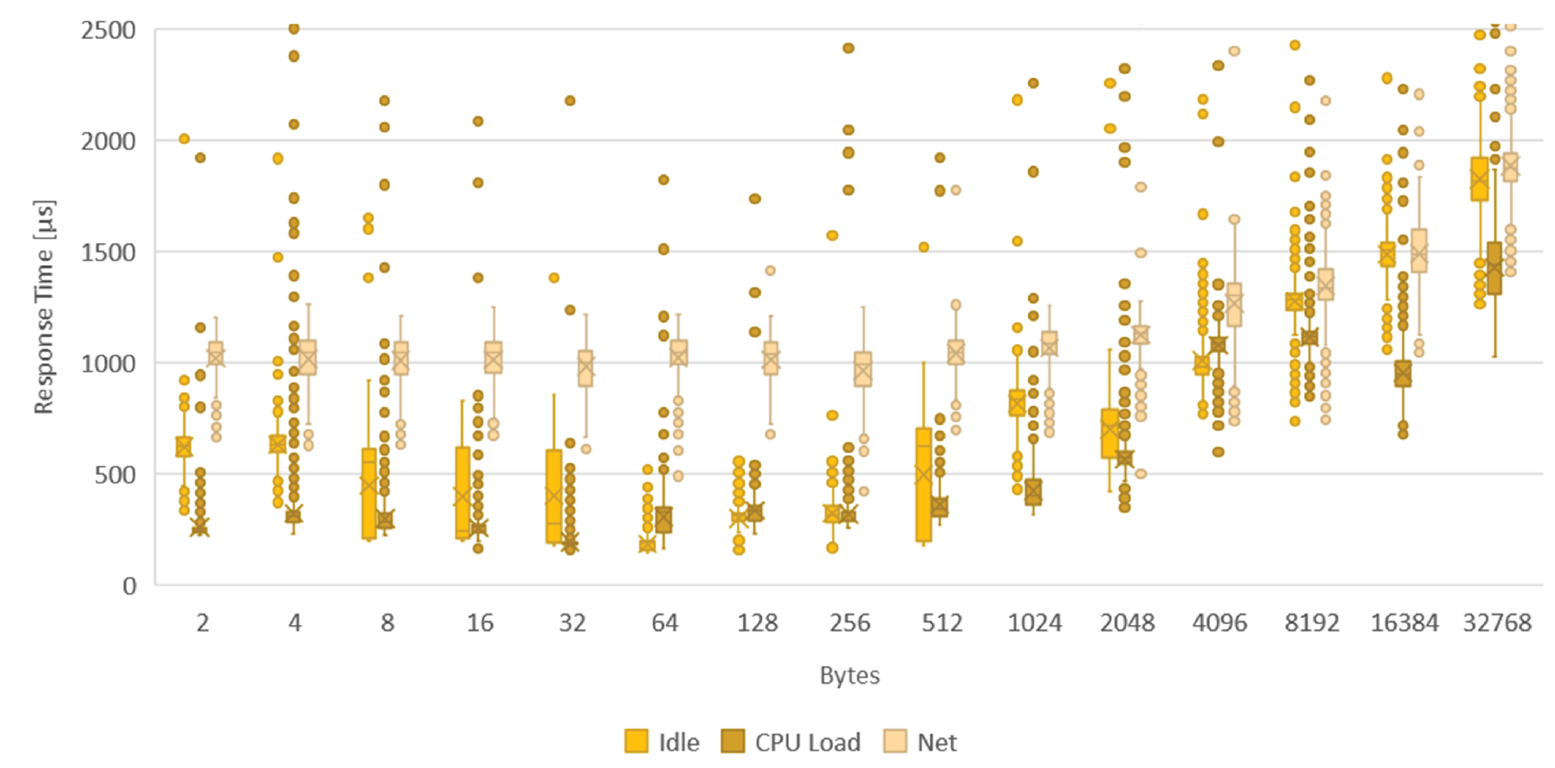
\includegraphics[width=\textwidth]{Bilder/ROS1Perform.PNG}
%		\caption{Echo \ac{RTT} in $[\mu s]$ of data messages in \ac{ROS} from 2 bytes to 32 kbytes by \cite{ROSPerform}.}
%		\label{fig_ROS1Perform}
%	\end{subfigure}
%	\hfill
%	\begin{subfigure}[b]{0.49\textwidth}
%		\centering
%		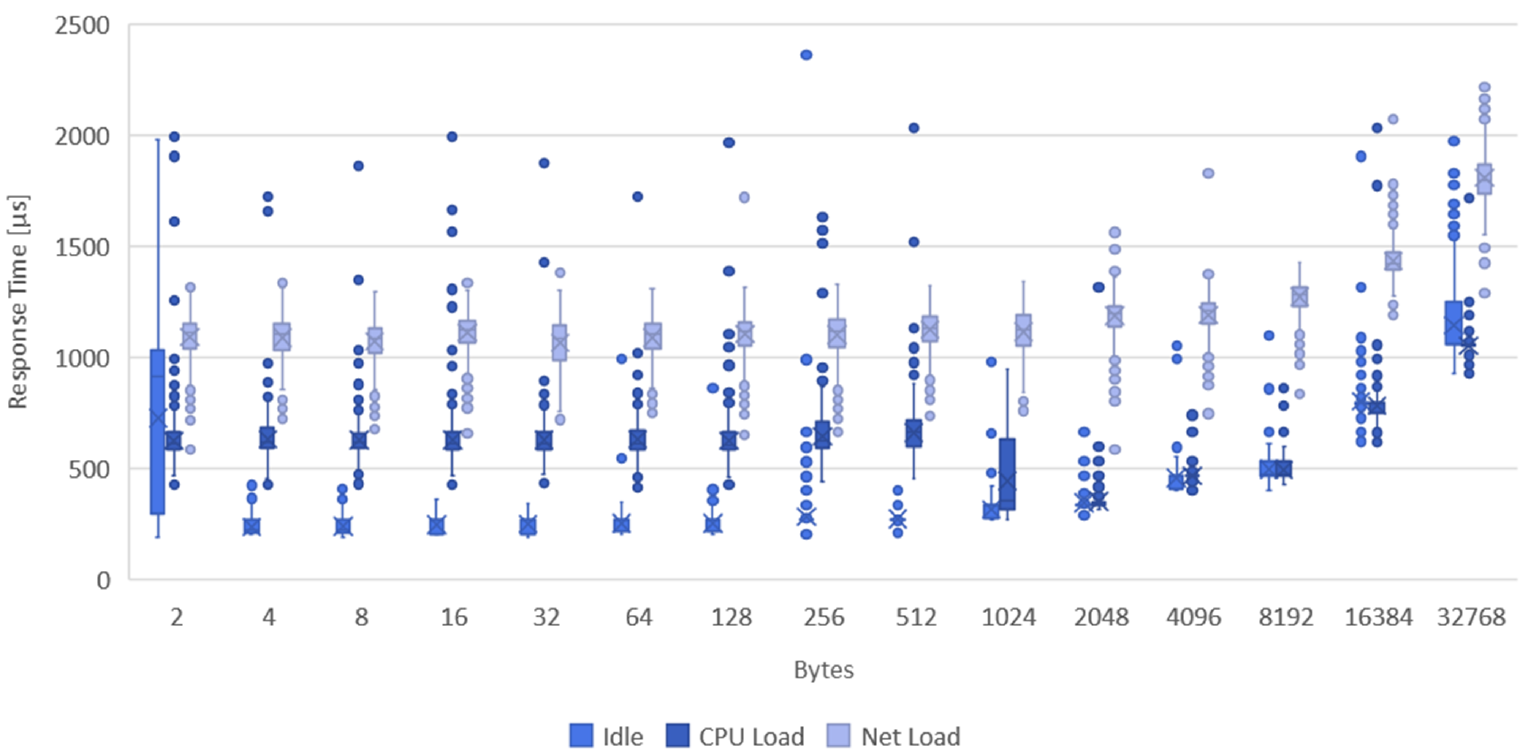
\includegraphics[width=\textwidth]{Bilder/DDSPerform.PNG}
%		\caption{Echo \ac{RTT} in $[\mu s]$ of data messages with \ac{DDS} from 2 bytes to 32 Kbytes by \cite{ROSPerform}.}
%		\label{fig_DDSPerform}
%	\end{subfigure}	
	\caption{ROS data transmission performance.}
	\label{fig_ROSPerform}
\end{figure}
\subsection{Virtual Environment} \label{virtuenv}
Virtual environments has been long used in the development of robotics to test new concepts, strategies and algorithms \cite{Gazebo}. With the inherent limitations of a real world testing environment such as unpredictable weather phenomena, wind induced currents and wakes and time dependent changes of light, simulated environments can increase the availability of suitable test variables, to name one advantage. There are many software solutions to simulate environments, however, especially in the field of \ac{USV}, using the simulation software Unity3D is a viable choice and can be preferred to other simulation software \cite{UnityUSV}. Unity3D is a game engine developed by Unity Technologies and allows for easy development of interactive scenes with a high visual fidelity. An asset store in which a large community  publish textures, models and extensions and other types of predefined assets makes the development process of a new scene efficient. Compared to most other simulation environments, the elements of the virtual environment built with Unity3D are close to the actual environment with an example given by an available high fidelity virtual water surface environment. Furthermore, virtual sensors can be modelled and embedded into the scene through scripts \cite{UnityUSV}. Unity features a powerful PhysX physics engine, a render engine and collision detection engine among others. Of special interest is that there is available a library called \textit{rosbridgelib} for Unity, that links the architectures of \ac{ROS} and Unity by using a \ac{JSON} data format to exchange messages \cite{ROStoUnity}. It has to be noted that this library is officially only implemented for ROS1 and planned only in 2022 for ROS2 as of information in 2021. However, as the message exchange format between ROS1 and ROS2 only differs in specific use cases, the library can as well be used for ROS2.

\section{Module Design}\label{ModuleDes}
% Describe the packages and messages used in ROS and the designstructure in Unity.

\begin{figure}[h]
	\centering
	\begin{tikzpicture}
	[node distance = 1cm, auto,font=\footnotesize,
	% STYLES
	every node/.style={node distance=3cm},
	% The comment style is used to describe the characteristics of each force
	comment/.style={rectangle, inner sep= 5pt, text width=4cm, node distance=0.25cm},
	% The force style is used to draw the forces' name
	force/.style={rectangle, draw, fill=black!10, inner sep=5pt, text width=2cm, text badly centered}]
	
	\node [rectangle, draw, fill=black!10, inner sep=5pt, text width=1cm, text badly centered] (Node) {Node.js};
	
	% Box Unity3d with comment
	\node [rectangle, left= 0.5cm of Node, draw, fill=black!5, minimum height=5cm, minimum width=6cm, dashed ] (Unity3d)         {};
	\node [comment, below=-0.5 of Unity3d, text centered]                                 (comment-Unity3d) {Unity3d Scene};
	
	% Boxes right inside Unity3d Scene
	\node [force, right=-2.75cm of Unity3d] (Manager) {Sensor Manager};
	\node [force, above = 0.5cm of Manager] (Sensor)  {Sensor Scripts};
	\node [force, below = 0.5cm of Manager] (ROS)     {ROS\#};
	
	% Boxes left inside Unity3d Scene
	\node [force, left=-2.75 cm of Unity3d] (Vessel) {Gameobject Vessel};
	\node [force, above = 0.5cm of Vessel]  (UI)     {User Interface};
	\node [force, below = 0.5cm of Vessel]  (Input)  {Input Script};
	
	% Links in Unity3d box
	\path[->,thick]

	(Vessel) edge (Sensor)
	(Input) edge (Vessel)
	(Sensor) edge (Manager)
	(Manager) edge (ROS);
	
	
	% ROS2 box with comment
	\node [rectangle, right=0.5cm of Node, draw, fill=black!5, minimum height=5cm, minimum width=6cm, dashed ] (ROS2){};
	\node [comment, below=-0.5 of ROS2, text centered]  (comment-ROS2) {ROS2 GNC System};
	
	% Guidance box with comment
	\node [rectangle, right=0.5cm of Node, draw, fill=black!5, minimum height=0.9cm, minimum width=5.5cm, dashed ] (Guid){};
	\node [comment, above=-0.2 of Guid, text centered]  (comment-Guid) {Guidance Subsystem};
	
	% Navigation box with comment
	\node [rectangle, above =0.5cm of Guid, draw, fill=black!5, minimum height=0.9cm, minimum width=5.5cm, dashed ] (Navi){};
	\node [comment, above=-0.2 of Navi, text centered]  (comment-Navi) {Navigation Subsystem};
	
	% Control box with comment
	\node [rectangle, below =0.5cm of Guid, draw, fill=black!5, minimum height=0.9cm, minimum width=5.5cm, dashed ] (Control){};
	\node [comment, above=-0.2 of Control, text centered] (comment-Control) {Control Subsystem};
	
	% Boxes inside Navigation, Guidance, Control
	\node [force, left=-2.5 cm of Navi]    (Process) {Processing};
	\node [force, right=-2.5 cm of Navi]   (Fusion)  {(Fusion)};
	
	\node [force, left=-2.5 cm of Guid]    (Map) 	 {Mapping};
	\node [force, right=-2.5 cm of Guid]   (Traject) {Trajectories};
	
	\node [force, left=-2.5 cm of Control] (Control) {Control};
	
	% Links to node.js
	\path[->,thick]
	(ROS) edge (Node)
	(Node) edge (Process)
	(Control) edge (Node)
	(Node) edge (ROS);	
	
	\end{tikzpicture} 
	\caption{Modules of the proposed system}
	\label{fig_modules}
\end{figure}

With the tools set according to the requirements, the module design takes place as depicted in figure \ref{fig_modules}. With a focus on the virtual environment, physical sensors are left out of the figure but can as well be integrated in conjunction with or in place of the virtual sensors. Figure \ref{fig_modules} is divided into two main components that are connected with the \ac{ROS} webbridge which is implemented in Node.js. Node.js is an asynchronous event-driven JavaScript runtime environment with the purpose of building scalable network applications. The Unity3d Scene to the left of the Node.js component is composed of a User Interface with which preferences to the Unity Scene such as the screen resolution can be chosen. An input script enables the user to send steering information via keyboard to the virtual vessel which is a Unity3d Gameobject and thus the position of the vessel can be manipulated. Assigned to the vessel are the scripts that simulate the sensors. The scripts send its data to a central Sensor Manager where the data structures are defined with which the data of the sensors can be send with the ROS\# to the \ac{ROS} webbridge. With the introduction of a Sensor Manager, sensors of different types can be easily integrated into the scene and its data types manipulated without changing definitions at various places inside the Unity3d Scene editor.\\ 

With the virtual environment set, the ROS2 component right to the Node.js component is required to receive the sensor data and manipulate it. This is done in three main categories of functions that are set up according the the specification of a \ac{GNC} system. First the Navigation Subsystem processes the received data. As the sensor data, particularly when transmitted combined, can amount to a high data rate, it is advantageous to process them directly in the procedure that receives the data.
After processing the data by filtering, feature extraction and clustering, the results of the different procedures can be fused into a fault resistant representation of the scene. With this representation, the Guidance Subsystem creates a map and calculates trajectories. The points prescribed by the trajectory are then used by the Control Subsystem to generate steering information either for a physical or a virtual implementation of the vessel. As required, the results of the processes inside the categories have to be visualized to the user, so that decisions of the system are understandable.

